\documentclass[sigconf,nonacm]{acmart}
\usepackage{xurl}
\setcopyright{none}
\settopmatter{printacmref=false,printfolios=true}
\renewcommand\footnotetextcopyrightpermission[1]{}
\acmConference{}{}{}
\acmDOI{}
\acmISBN{}
\citestyle{acmnumeric}
\title[AdaptiveAttend Milestone]{AdaptiveAttend: Scene-Adaptive Intervention Strength for 3D Foundation Models}
\subtitle{Project milestone, November 16, 2026}
\author{Eric Lu (NetID: yl4386)}
\author{Swati Parida (NetID: sp2735)}
\author{Anastasios Gerasis (NetID: ag2766)}
\renewcommand{\shortauthors}{AdaptiveAttend team}

\begin{document}
\begin{abstract}
ArchAttend steers frozen 3D reconstruction models toward architectural elements, but a single intervention strength may not suit every scene or model activation. We investigate adaptive intervention strengths without using ground-truth reconstruction at inference time. We reproduce a matched VGGT baseline on 39 development landmarks and study strength selection from Pass-1 signals. No tested Pass-1 selector outperforms the best fixed strength under cross-validation. A depth-drift selector detects most large-step failures but does not beat the fixed strength on its 40-scene test set. For layer-, view-, and anchor-dependent strengths, we construct and audit a 54-landmark development subset with separate calibration and confirmation splits. On 36 confirmation landmarks, layer-dependent strength improves mean normalized Chamfer error over the calibrated scalar and wins on 23 landmarks; view-dependent strength wins on 13 and slightly worsens the mean. Neither improves mean error over no intervention. The anchor-dependent experiment remains unfinished. Final-stage evaluation will cover all 396 landmarks while preserving a separate 79-landmark test partition.
\end{abstract}
\keywords{3D reconstruction, attention intervention, inference-time adaptation, adaptive step size}
\begin{teaserfigure}
\centering
{\small\shortstack[c]{\textbf{Project repository (GitHub):}
\href{https://github.com/swati1504/ArchWorld}{\textcolor{blue}{\nolinkurl{https://github.com/swati1504/ArchWorld}}}\\
Structured experiments:
\href{https://github.com/tasosger/ArchWorld/tree/point3/hypothesis-notebooks}{\textcolor{blue}{notebooks and run instructions}}
\quad\href{https://github.com/swati1504/ArchWorld/pull/4}{\textcolor{blue}{PR \#4 (pending merge)}}}}\\[0.6em]
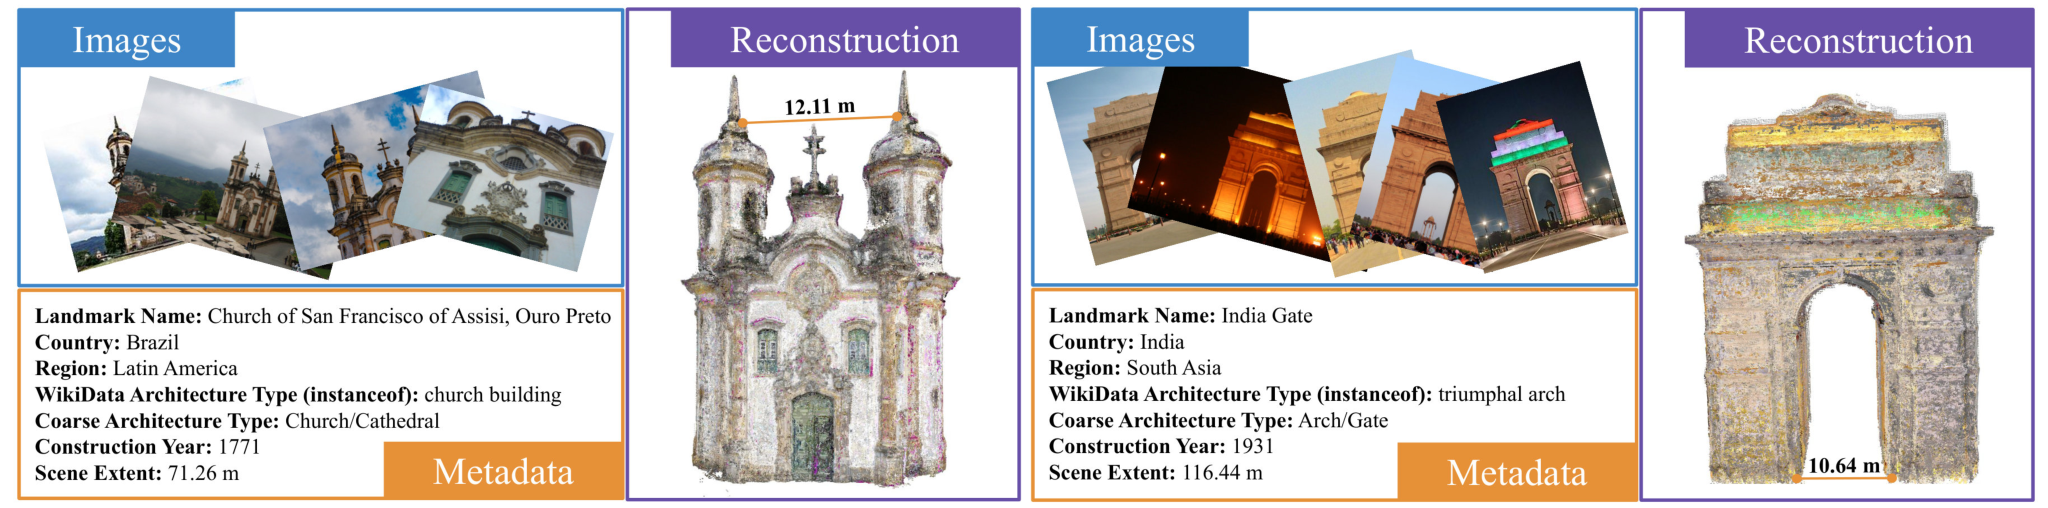
\includegraphics[width=\textwidth]{figures/archworld_photos.png}
\caption{Landmark photographs and corresponding benchmark reconstructions: Church of San Francisco of Assisi in Ouro Preto (left) and India Gate (right). Reproduced from Kriplani et al.~\cite{archworld}, Figure 2, under \href{https://creativecommons.org/licenses/by/4.0/}{CC BY 4.0}. These illustrate the dataset, not new AdaptiveAttend outputs.}
\Description{Photographs of a church in Brazil and India Gate show changes in viewpoint, lighting, and surroundings. Each set is paired with a dense reconstruction and scene metadata in the source figure.}
\label{fig:photos}
\end{teaserfigure}
\maketitle

\section{Problem and research basis}
VGGT~\cite{vggt} predicts scene geometry from multiple images in a feed-forward model. Our investigation builds on ArchWorld and ArchAttend~\cite{archworld}, which study architectural reconstruction across geographic regions and introduce an inference-time attention intervention. The intervention changes intermediate token representations while keeping model weights frozen. Our research question is: \emph{can we choose intervention strength from a scene's predicted geometry, approaching the best tested strength without accessing that scene's ground-truth reconstruction?}

The strength $\eta$ controls the size of the activation update. A small value may have little effect, while a large value may damage the reconstruction. Choosing the best strength using ground truth provides an oracle comparison, but is unavailable when reconstructing a new scene. The project combines baseline evaluation, scene-level strength selection, and structured intervention rules. The benchmark, pretrained backbone, supplied anchor choices, and reference intervention are inherited components. The shared project repository provides the implementation context~\cite{teamrepo}.

\paragraph{Code and reproducibility.}
The public team repository is \url{https://github.com/swati1504/ArchWorld}. The structured-intervention code, three hypothesis notebooks, shared mask workflow, and run instructions are available in the \href{https://github.com/tasosger/ArchWorld/tree/point3/hypothesis-notebooks}{experiment branch} (commit \texttt{92d9149})~\cite{point3}. \href{https://github.com/swati1504/ArchWorld/pull/4}{Pull request \#4} proposes merging this branch into the team repository; it is pending as of November 16, 2026.

\section{Formal task, data, and evaluation}
For scene $s$, let $X_s=\{I_{s,v}\}_{v=1}^{V_s}$ be its images, $M_s$ the anchor segmentation masks, and $G_s$ its ground-truth point cloud. A frozen model with intervention strength $\eta$ produces reconstructed points $P_s(\eta)$. An adaptive rule may use images, masks, model activations, or predictions to determine strength. Its parameters may be calibrated on development scenes, but inference for a new scene must not use $G_s$.

\paragraph{Data and split.}
ArchWorld contains 396 landmarks across eight geographic regions, with architecture metadata and metric-scale ground truth~\cite{archworld}; Figure~\ref{fig:photos} shows example photos and reconstructions. The structured-intervention study uses a frozen partition of 317 training/development landmarks and 79 held-out landmarks. Its 54-landmark development subset is constructed as described in Section~\ref{sec:point3}; no held-out landmark enters subset selection or calibration.

\paragraph{Reconstruction error.}
After the pipeline's alignment and validity filtering, we measure symmetric Chamfer distance using unsquared Euclidean distances:
\begin{equation}
\begin{aligned}
\mathrm{CD}(P,G)={}&\frac{1}{2|P|}\sum_{p\in P}\min_{g\in G}\|p-g\|_2\\
&+\frac{1}{2|G|}\sum_{g\in G}\min_{p\in P}\|g-p\|_2.
\end{aligned}
\label{eq:cd}
\end{equation}
The two terms are reconstruction accuracy and completeness. The repository also reports metric distance $\mathrm{CD}_{m,s}=\mathrm{Scale}_s\,\mathrm{CD}_s$ and extent-normalized distance
\begin{equation}
\mathrm{CD}_{\mathrm{norm},s}=1000\,\mathrm{CD}_{m,s}/\mathrm{Extent}_s,
\end{equation}
where extent is in metres. Lower values are better. The structured-intervention study compares paired normalized-CD differences and weights landmarks equally.

\section{Reference Intervention}
\begin{figure*}[t]
\centering
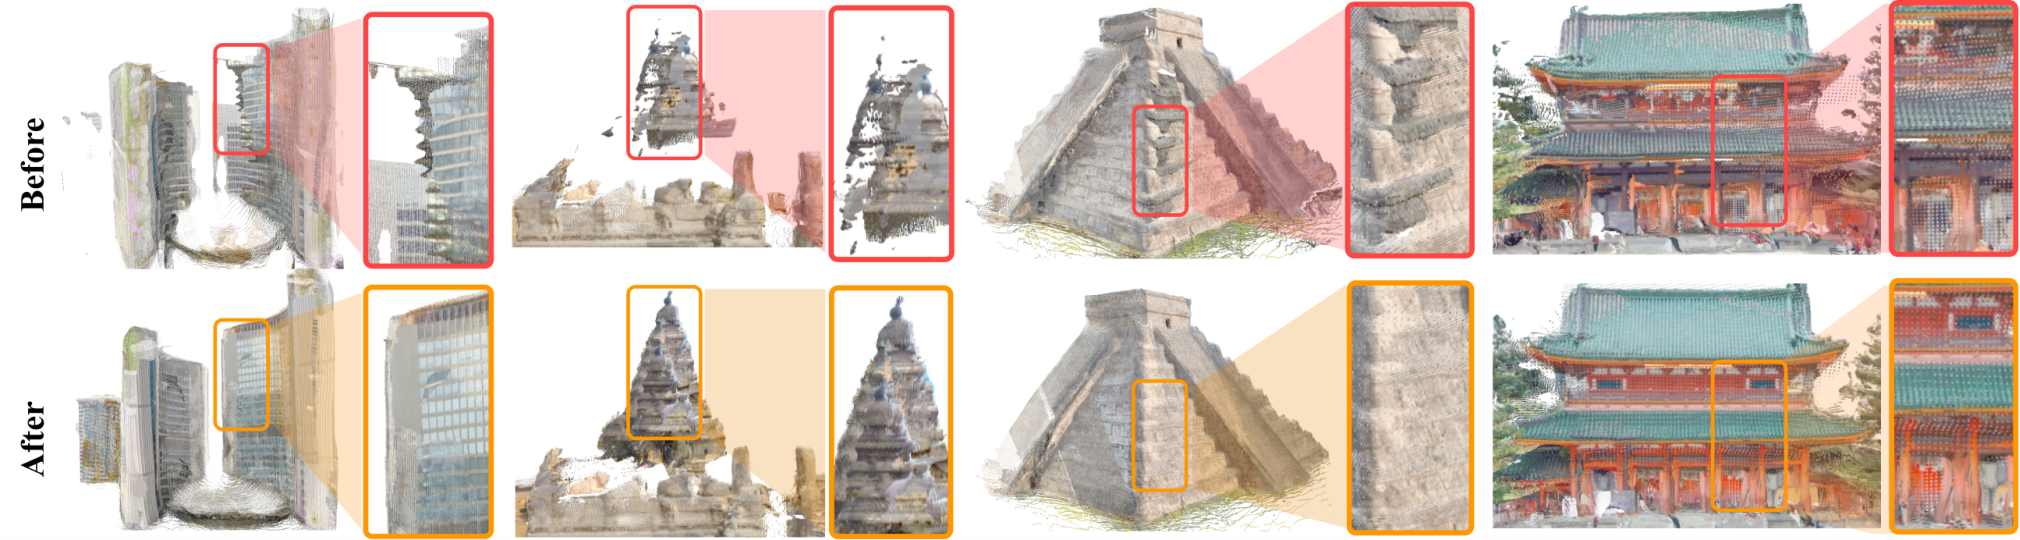
\includegraphics[width=\textwidth]{figures/archattend_reconstructions.png}
\caption{Prior-work reconstruction examples before (top) and after (bottom) ArchAttend: Toronto City Hall, Shore Temple, Chichen Itza, and Heian-jingu. Reproduced from Kriplani et al.~\cite{archworld}, Figure 7, under \href{https://creativecommons.org/licenses/by/4.0/}{CC BY 4.0}. These are the original authors' results, not outputs from our adaptive selector.}
\Description{Four side-by-side landmark reconstruction comparisons show the original paper's before and after rows. Colored boxes highlight filled surfaces and reduced duplicate structures.}
\label{fig:prior-reconstructions}
\end{figure*}
Figure~\ref{fig:prior-reconstructions} illustrates the original intervention's qualitative motivation. Our shared experiments use the supplied architectural anchor $e_s^*$ and its SAM 3 masks, rather than repeating anchor selection. At each global attention layer $l\in\{0,\ldots,23\}$, the inherited VGGT hook computes a scaled, normalized attention objective $J_l$ for the anchor and proposes
\begin{equation}
\widetilde T_s^l=T_s^l+\eta\nabla_{T_s^l}J_l(T_s^l,M_s).
\label{eq:update}
\end{equation}
For one scene, the default masked mean objective can be written as $J_l=c\,(H m^2)^{-1}\sum_{h,i,j}M_iM_j A^l_{hij}$, where $A^l$ is the hook's attention matrix, $H$ is the head count, $M_i$ indicates an anchor token, $m=\sum_iM_i$, and $c=10^5$. The hook retains an update only when its monitored anchor-attention statistic increases; otherwise it restores the previous tokens. We retain the inherited objective scaling and attention conventions, because changing them would change the meaning of $\eta$.

\section{Baseline Implementation and Evaluation}
\label{sec:eric}
% ===== BEGIN Eric: baseline =====
Every reported gain from ArchAttend is a comparison against unmodified VGGT, so the comparison is only meaningful if both arms are scored by the same pipeline. This section reproduces that no-intervention arm on the 39 landmarks of the shared development list (\texttt{scenes\_dev.txt}). This list is separate from the structured-intervention subset in Section~\ref{sec:point3}. Each landmark contributes the benchmark views that have ground-truth depth: 42--50 views for 38 landmarks and 21 for one.

Let $C_s(\eta)$ denote $\mathrm{CD}_{\mathrm{norm},s}$ of $P_s(\eta)$. The baseline is $C_s(0)$: we run the reference intervention pipeline at $\eta=0$. The update in Equation~\ref{eq:update} is then zero, so the accept/revert rule restores the original tokens and the prediction is exactly that of unmodified VGGT, scored by the same code as the team's $\eta$ sweep. Settings match the sweep: fp32 weights, the built-in pre-intervention pass skipped to fit memory, ICP refinement after RANSAC alignment, and prediction filtering with the dataset's manual filtration masks. All runs use one NVIDIA L4 (24\,GB). Following the reference aggregation, we report the median of $C_s$ over landmarks and the per-landmark change $\Delta_s(\eta)=C_s(\eta)/C_s(0)-1$.

\begin{table}[htb]
\caption{No-intervention VGGT on the 39 development landmarks (median $\mathrm{CD}_{\mathrm{norm}}$, lower is better). The paper value covers all 396 landmarks.}
\label{tab:eric-base}
\centering
\begin{tabular}{lr}
\toprule
Configuration & Median\\
\midrule
$\eta=0$, sweep pipeline (ours) & 3.89\\
$\eta=1$, team sweep & 3.85\\
Best $\eta$ per scene (oracle) & 3.63\\
Benchmark script (no filter/ICP) & 20.13\\
Paper~\cite{archworld}, 396 landmarks & 3.28\\
\bottomrule
\end{tabular}
\end{table}

\paragraph{A first attempt that was not comparable.} We first used the standalone benchmark script. All 39 landmarks completed, but the median was 20.13 (Table~\ref{tab:eric-base}). By default this script neither filters predictions to the landmark nor applies ICP, and our run used bf16 weights. Missing filtering explains most of the gap: on one landmark, enabling it alone reduced $\mathrm{CD}_{\mathrm{norm}}$ from 110.1 to 4.43. We keep this number only as a benchmark-script reference, not as the ``before'' arm.

\paragraph{Reproduced baseline.} Through the sweep pipeline, all 39 landmarks completed with a median of 3.89, close to the paper's 3.28, which covers all 396 landmarks rather than this subset. The baseline agrees with the team's $\eta=1$ run, the smallest tested step: their per-landmark ratio has median 0.998, and the two rank landmarks almost identically (Spearman 0.997, compared with 0.63 for the benchmark-script run).

\paragraph{How much the intervention helps.} Relative to $\eta=0$, choosing the best $\eta$ per landmark gives a median per-landmark relative reduction of 3.0\% (mean 5.6\%). It improves 16 landmarks by more than 5\%; on 4 landmarks every tested $\eta$ is worse than no intervention. Among fixed strengths, only $\eta=1000$ differs significantly from $\eta=0$: median $-1.2\%$, better on 27 of 39 landmarks, $p=0.046$.
% ===== END Eric: baseline =====

\section{Predicting \texorpdfstring{$\eta$}{eta} from Pass-1 Signals}
\label{sec:eric-pass1}
% ===== BEGIN Eric: Point 2 =====
This section addresses one direction of adaptive selection: predicting $\eta$ from signals that ArchAttend already computes in Pass~1, before any intervened forward pass. Pass~1 is an ordinary forward pass that selects the anchor $e_s^*$, the architectural element with the highest semantic cross-view attention (SCVA)~\cite{archworld}. If the same pass also indicates how strong a step a landmark can take, the five-way oracle sweep could be replaced by a single prediction made without $G_s$.

\paragraph{Task and evaluation.} Let $E=\{1,10,100,1000,5000\}$, the sweep grid, and $C_s(\eta)$ as in Section~\ref{sec:eric}, taken from the team's sweep on the same 39 landmarks. A selector $\pi$ maps a Pass-1 feature vector $\phi_s$ to $\pi(\phi_s)\in E$. Here $\phi_s$ depends only on $X_s$, $M_s$ and the attention of one unintervened forward pass. Performance is measured by the regret
\begin{equation}
R_s(\eta)=\frac{C_s(\eta)}{\min_{\eta'\in E}C_s(\eta')}-1,
\label{eq:regret}
\end{equation}
which is zero when the oracle strength is chosen. With leave-one-landmark-out cross-validation, $\pi^{(-s)}$ is fitted on the other 38 landmarks and we record $R_s(\pi^{(-s)}(\phi_s))$. We report mean regret, the number of landmarks with regret above 10\%, and the reference convention's median change in $C_s$. The reference rules are a fixed $\eta=1$, the best fixed $\eta$ chosen on the training folds only, and the oracle.

\paragraph{Pass-1 signals.} The proposal names three candidate signals: attention entropy, the anchor's SCVA, and attention leakage onto non-architectural elements. We extract all three, plus anchor coverage. SAM~3 masks cover every architectural element listed for the landmark and eight non-architectural labels (sky, tree, bush, grass, water, person, car, road). A $14{\times}14$ patch is assigned to element $e$ when more than half of it is covered by $e$'s mask. Let $P_e$ be these patches, $P_{e,v}$ those in view $v$, and $\bar A^l$ the head-averaged attention at global layer $l\in\{0,\ldots,23\}$. We compute SCVA in the form written in the paper,
\begin{equation}
S^{\mathrm{eq}}_l(e)=\sum_{i\in P_e}\sum_{j\in P_e}\bar A^l_{ij},
\end{equation}
and in the form used by the reference code, which keeps only pairs from different views and averages within each view pair,
\begin{equation}
S^{\mathrm{code}}_l(e)=\sum_{u\neq v}\frac{1}{|P_{e,u}||P_{e,v}|}\sum_{i\in P_{e,u}}\sum_{j\in P_{e,v}}\bar A^l_{ij}.
\end{equation}
Each form is computed with and without rotary position encoding, and the anchor is $e_s^*=\arg\max_e S_{23}(e)$ over architectural elements. From the same pass we derive per-layer anchor SCVA, attention entropy $H_l=\operatorname{mean}_i\bigl(-\sum_j\bar A^l_{ij}\log\bar A^l_{ij}\bigr)$, and the share of anchor-token attention that lands on non-architectural tokens. Anchor coverage is measured as the patch share $\rho^{\mathrm{patch}}_s=|P_{e^*}|/\sum_v N_v$ and the view share $\rho^{\mathrm{view}}_s$, the fraction of views containing the anchor. In total there are 88 scene-level features.

\paragraph{Selectors.} We compare: ridge regression on $\log_{10}\eta^*_s$, snapped to $E$; a nearest-neighbour rule that averages the regret curves of the ten closest training landmarks and picks their minimum; rules based on metadata (region, building type, anchor type, construction year, view count); and a threshold rule on anchor coverage. The threshold rule picks a cut-off $\tau$ inside each training fold, then assigns each side its own best $\eta$ from $E$. The anchor-coverage hypothesis and its test were recorded in the project log before the test was run. A permutation test with shuffled features checks each selector against chance.

\begin{table}[htb]
\caption{Fixed-strength selectors on the 39 development landmarks. Regret follows Equation~\ref{eq:regret}; ``best on'' counts landmarks where that $\eta$ is the oracle.}
\label{tab:eric-regret}
\centering
\begin{tabular}{lrr}
\toprule
Fixed $\eta$ & Mean regret & Best on\\
\midrule
1 & 7.6\% & 4\\
10 & 8.1\% & 5\\
100 & 7.4\% & 7\\
1000 & \textbf{4.4\%} & 7\\
5000 & 38.9\% & 16\\
Oracle & 0 & 39\\
\bottomrule
\end{tabular}
\end{table}

\paragraph{The bar to beat.} The oracle strength varies by landmark (Table~\ref{tab:eric-regret}). Chosen on training folds, the best fixed strength is $\eta=1000$ in every fold, with 4.4\% mean regret. Although $\eta=1000$ is the oracle on only 7 landmarks, it is within 5\% of the oracle on 29. In contrast, $\eta=5000$ is the oracle most often but is up to $6.3\times$ worse than the best strength elsewhere.

\paragraph{Pass~1 is reproduced.} With $S^{\mathrm{code}}$, our recomputed anchors match the supplied anchors on 34 of 39 landmarks; with $S^{\mathrm{eq}}$, they match on only 17. The supplied anchors therefore follow the code's definition, not the paper's equation, which favours large elements. Rotary position encoding never changes the selected anchor. Four of the five mismatches are near-ties, where the supplied anchor reaches 85--99\% of our winner's score.

\paragraph{No selector beats the fixed strength yet.} No metadata rule (all correlations $p\ge0.09$) and no selector built on the 88 features beats $\eta=1000$. The strongest single correlate of $\eta^*_s$ is layer-4 attention entropy (Spearman $\rho=-0.47$, $p=0.003$): landmarks with more diffuse early attention prefer smaller steps. With 88 features tested, however, a correlation of this size can arise by chance.

\paragraph{Anchor coverage predicts large-step failures.} As hypothesised before the test, smaller anchors make $\eta=5000$ worse: $\rho=-0.41$ ($p=0.010$) for patch share and $\rho=-0.40$ ($p=0.012$) for view share. The relationship still holds when the landmark that inspired the hypothesis is removed ($\rho\approx-0.35$, $p\approx0.03$). On the six landmarks where $\eta=5000$ fails worst, the anchor covers a median 0.7\% of patches and appears in 68\% of views, compared with 8\% and 98\% elsewhere. Turned into a decision rule, however, coverage does worse than the fixed strength under cross-validation (7.9\% and 7.1\% mean regret, against 4.4\%) and is indistinguishable from shuffled features ($p\approx0.4$--$0.5$). Only about six landmarks show the failure, so the learned cut-off depends heavily on which of them are in the training fold.

\paragraph{Limitations and next steps.} In these 39-landmark runs, the alignment step before scoring uses an unseeded random generator, so repeated scorings of the same prediction differ by a few percent. That is comparable to the gap between the best and second-best $\eta$ on many landmarks, so some ``best $\eta$'' labels are partly chance, and the negative result above does not yet show that Pass-1 signals are uninformative. Next, we will (i) re-derive the labels with fixed seeds and several scoring draws per run, (ii) repeat the feature ranking and selector comparison on these labels, and (iii) confirm the strongest signals on development landmarks not used so far.
% ===== END Eric: Point 2 =====

\section{Adaptive Strength Selection and Analysis}
\label{sec:swati}
This section uses a separately constructed 39/40 development/test split. Its ratio regret uses 1 for the oracle, whereas the excess regret in Equation~\ref{eq:regret} uses 0; candidate sets are specified below. This part addresses scene-level selection by optimizing an unsupervised proxy objective at inference time: for each scene we run a small set of candidate strengths and choose among them using only the model's own outputs.

\paragraph{Setup.} We use VGGT-1B with the hook on layers 0--23, the 50 benchmark views per scene, and fp32 on one NVIDIA L4 (24\,GB); the separate base pass is skipped so that the intervention fits in memory. We sweep $\eta\in\{1,10,100,1000,5000\}$ on 39 development scenes and keep 40 held-out test scenes. Because the full benchmark did not fit on our disk, we drew a random sample of 80 landmarks stratified by region (proportional to each region's size, at least one per region, seed 0) and split it into 40 development and 40 test scenes; one development scene is missing from the benchmark's view list and was dropped, leaving 39. The same development list is used for the baseline in Section~4. Test scenes were not run until the rule below was frozen. Scores come from the pipeline of Section~3 (alignment with ICP and filtration masks). We report the regret $R_s=\mathrm{CD}_s(\hat\eta_s)/\min_{\eta}\mathrm{CD}_s(\eta)$, where $1$ means the best tested strength was chosen and a scene with $R_s>1.2$ counts as a failure. Because $\mathrm{CD}_{\mathrm{norm},s}$ is $\mathrm{CD}_s$ times a per-scene constant, regret is the same under either metric.

\paragraph{What the sweep shows.} No single strength is safe. $\eta=5000$ is the best tested strength on 16 of 39 development scenes but has the worst mean error, because it breaks 7 reconstructions (worst regret 6.25). $\eta=1000$ has the best mean (mean regret 1.044) but misses the gains on scenes where 5000 helps.

\paragraph{Label-free signals.} For every candidate we compute four quantities without $G_s$: mean log depth confidence; multi-view consistency of depth reprojected with the predicted cameras; depth drift $\delta_s(\eta)$, the median relative change in predicted depth compared with the $\eta=1$ run; and the change in predicted camera rotations. Drift captures the failure mode directly: when a large step breaks a scene, the geometry moves away from the nearly unmodified prediction. On development scenes, $\delta_s(5000)$ correlates with the regret of $\eta=5000$ (Spearman 0.58), rotation drift less so (0.35), and choosing the most confident output does worse than a fixed $\eta=1000$ (mean regret 1.076).

\paragraph{Selection rule.} We take the largest strength whose drift stays below a threshold:
\begin{equation}
\hat\eta_s=\begin{cases}5000 & \text{if } \delta_s(5000)\le\tau,\\ 1000 & \text{otherwise,}\end{cases}
\label{eq:drift-rule}
\end{equation}
with $\tau=0.00626$ chosen by leave-one-out on the development scenes and then frozen. The rule needs the $\eta=1$ and $\eta=5000$ passes, plus the $\eta=1000$ pass when it falls back. Variants that searched more of the grid (largest $\eta$ under the threshold, and a drift-ratio rule) did not improve on it.

\begin{table*}[t]
\caption{Scene-level strength selection. Development regret is against the best of all five tested strengths (leave-one-out $\tau$); test regret is against the better of $\eta=1000$ and $\eta=5000$, the two values the rule chooses between. Failures are scenes with regret above 1.2. Mean CD is over the 40 test scenes.}
\label{tab:drift}
\small
\begin{tabular}{lccc|cccc}
\toprule
 & \multicolumn{3}{c|}{Development (39 scenes)} & \multicolumn{4}{c}{Held-out test (40 scenes)} \\
Selector & Mean regret & Worst & Failures & Mean regret & Worst & Failures & Mean CD \\
\midrule
Fixed $\eta=1000$ & 1.044 & 1.22 & 1 & \textbf{1.017} & 1.11 & 0 & \textbf{0.0632} \\
Fixed $\eta=5000$ & 1.389 & 6.25 & 7 & 1.545 & 18.67 & 6 & 0.0735 \\
Most confident output & 1.076 & 2.14 & 4 & -- & -- & -- & -- \\
Drift rule (Eq.~\ref{eq:drift-rule}) & \textbf{1.037} & 1.22 & 1 & 1.033 & 1.65 & 1 & 0.0641 \\
Oracle & 1.000 & 1.00 & 0 & 1.000 & 1.00 & 0 & 0.0623 \\
\bottomrule
\end{tabular}
\end{table*}

\begin{figure}[t]
\centering
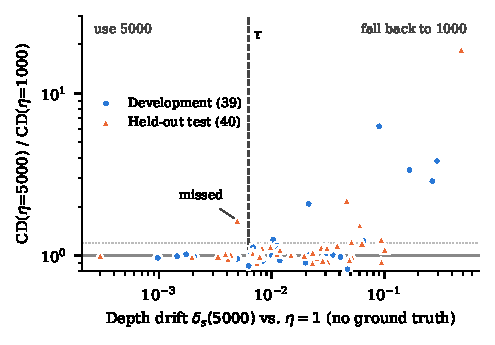
\includegraphics[width=\columnwidth]{figures/drift_vs_regret.pdf}
\caption{Depth drift at $\eta=5000$ (computed without ground truth) against how much worse $\eta=5000$ is than $\eta=1000$, per scene. Each point is a scene; the dashed line is the frozen threshold $\tau$. Scenes where the large step breaks the reconstruction have high drift, so the rule falls back to $\eta=1000$; the one test scene it missed is marked. The dotted line marks 20\% worse. One test scene with zero drift is drawn at the left edge.}
\Description{Scatter plot on log axes. Horizontal axis is depth drift at step size 5000; vertical axis is the ratio of Chamfer distance at 5000 to that at 1000. Most scenes cluster near ratio 1 at all drift levels. Scenes with large ratios, up to about 19, sit to the right of the threshold line, except one test scene at ratio 1.65 just left of it.}
\label{fig:drift}
\end{figure}

\paragraph{Results.} Table~\ref{tab:drift} summarizes both splits. On development scenes the drift rule had the lowest mean regret of the selectors we tried, with 10 wins, 27 ties and 2 losses against fixed $\eta=1000$, but the difference was not significant (Wilcoxon $p=0.064$; paired bootstrap 95\% CI of the mean regret difference $[-0.018, 0.004]$). On the 40 held-out scenes the frozen rule chose $\eta=5000$ for 8 scenes and did not beat fixed $\eta=1000$: 4 wins, 33 ties and 3 losses, a mean change of $+1.5\%$ (Wilcoxon $p=1.0$). Almost all of the gap comes from one scene whose drift fell under the threshold while $\eta=5000$ was 65\% worse. The drift signal does work as a failure detector (Figure~\ref{fig:drift}): $\eta=5000$ is more than 20\% worse than $\eta=1000$ on 6 test scenes, and the rule falls back on 5 of them, including one where $\eta=5000$ is 18.7 times worse.

\paragraph{Interpretation.} The per-scene choice between the two useful strengths has little room to help. Even a perfect choice between $\eta=1000$ and $\eta=5000$ is only 1.4\% better than fixed $\eta=1000$ on the test scenes, and no threshold applied to the test set does better than the fixed setting, so the outcome is not caused by a poorly tuned $\tau$. That margin is smaller than the scoring noise: the alignment step uses unseeded random sampling, and rescoring an unchanged prediction moves a scene's CD by 2--15\%. Depth drift is therefore a reliable label-free signal that a large step has broken the reconstruction, but for selecting $\eta$ a fixed $\eta=1000$ is the practical choice, with the drift check as a safeguard when larger steps are used. Next steps are rescoring the saved predictions with seeded alignment to obtain cleaner labels, and combining drift with Pass-1 anchor statistics. Code and per-scene results are in the \texttt{swati/} folder of the team repository~\cite{teamrepo}.

\section{Structured Intervention Methodology}
\label{sec:point3}
We investigate strengths that vary by layer (H1), view (H2), or anchor (H3). The published implementation and selection audit are available~\cite{point3}. We select 54 of 317 training/development landmarks, excluding the 79 held-out landmarks. This subset reduces the GPU workload for repeated reconstructions, mask preparation, and hypothesis comparisons during development; final evaluation will use the whole dataset.

\begin{figure*}[t]
\centering
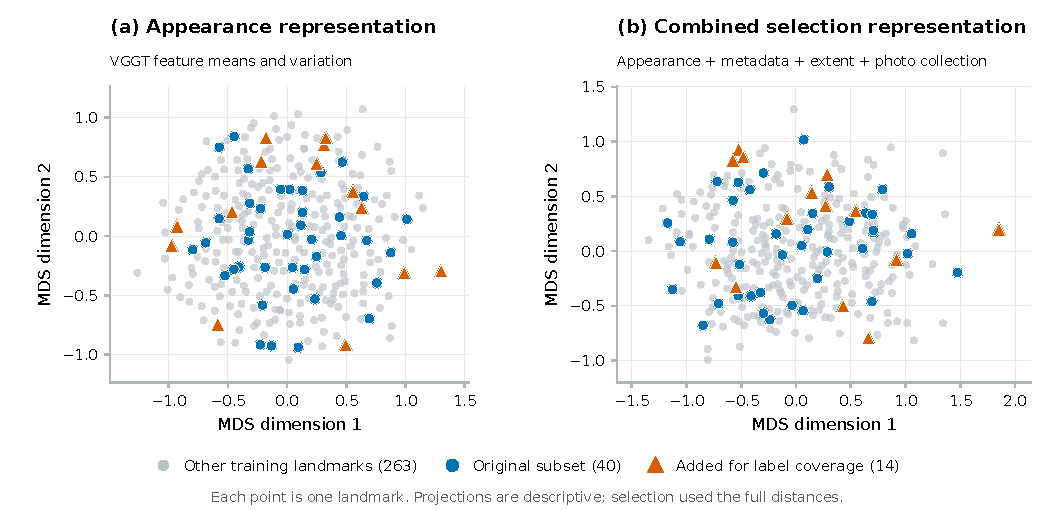
\includegraphics[width=\textwidth]{figures/point3_selection_representations.pdf}
\caption{Representations used to construct the structured-intervention subset. Left: distances from VGGT feature means and variation. Right: the combined appearance, metadata, extent, and photo-collection distance used by the selector. Gray points are the 263 unselected training landmarks; blue circles are the original 40; orange triangles are the 14 additions. Two-dimensional proximity is approximate. These are selection diagnostics, not reconstruction results.}
\Description{Two maps display the same 317 training landmarks in two-dimensional projections of their saved distances. The left map uses visual appearance descriptors; the right uses all four selection descriptor families. The selected 54 landmarks are distinguished from the remaining 263, with separate markers for the original 40 and 14 additions.}
\label{fig:representations}
\end{figure*}

\subsection{How the subset was generated}
We retain a frozen, previously selected set of 40 landmarks and add one for each of its 13 omitted named anchor labels plus the missing-label category. Each landmark has one supplied label, so these 14 additions are minimal while preserving the original 40. This does not establish 54 as an optimal representative sample size.

We enumerate all 336 possible combinations of these additions and minimize
\begin{equation}
Q(S)=0.35\bar d_S+0.35d_{95,S}+0.15\overline{\mathrm{TV}}_S+0.15\overline{\mathrm{KS}}_S.
\label{eq:subset}
\end{equation}
Here $d_S(x)=\min_{s\in S}D(x,s)$ measures distance to the closest selected landmark; its mean and 95th percentile exclude self-distances and use the 263 unselected training landmarks. $D$ equally weights four normalized families: full-image VGGT feature means/variation; type/region/anchor metadata; physical extent; and photo-collection count, duplicates, resolution, and aspect ratio. Normalization uses training landmarks only. The final terms average categorical total variation (TV) and numeric Kolmogorov--Smirnov (KS) distances over the three and four attributes in Table~\ref{tab:subset}. No reconstruction outcome or held-out image descriptor enters selection. This optimum is restricted to repairs of the original 40; proportional quotas are not enforced.

The audit records 14,333 source photographs. Selection preserves their identities; the reconstruction view limit is a separate step.

\subsection{How closely it matches the dataset}
For proportions, $\mathrm{TV}(p,q)=\tfrac12\sum_k|p_k-q_k|$; for empirical numeric distributions, $\mathrm{KS}(F,G)=\sup_t|F(t)-G(t)|$. Both range from zero (matching distributions) to one. Table~\ref{tab:subset} combines the training audit with a post-selection check against full-benchmark metadata. This check uses no held-out images or reconstruction outcomes and did not change selection.

\begin{table}[htb]
\caption{Distribution gaps between the 54-landmark subset and reference populations. Lower is closer. Dashes indicate that full-benchmark photo descriptors were not audited.}
\label{tab:subset}
\centering
\begin{tabular}{lrr}
\toprule
Attribute / distance & Training (317) & Full (396)\\
\midrule
Building type / TV & 0.0782 & 0.0774\\
Region / TV & 0.0331 & 0.0236\\
Supplied anchor / TV & 0.2017 & 0.1978\\
Extent / KS & 0.0444 & 0.0539\\
Image count / KS & 0.0983 & ---\\
Duplicate fraction / KS & 0.0612 & ---\\
Median megapixels / KS & 0.0721 & ---\\
\bottomrule
\end{tabular}
\end{table}

The subset covers all nine building types, eight regions, and 25 training anchor-label categories, including missing labels. Of the full benchmark's 27 anchor categories, gate and spire are absent. Region proportions are close; anchor proportions differ more because rare labels were deliberately included. Window labels account for 7.41\% of the subset and 13.56\% of training landmarks. Distance to the nearest selected landmark has mean 0.502 and 95th percentile 0.690 in normalized descriptor units. These diagnostics do not certify reconstruction performance, camera coverage, blur, or exposure, nor give a percentage of representativeness.

\subsection{Visualizing the selection representations}
Figure~\ref{fig:representations} projects the saved appearance and combined selection distances into two dimensions using metric multidimensional scaling (MDS). Each point is one of the 317 training landmarks; color and shape identify the original 40 and the 14 additions. The combined distance equally weights all four descriptor families. Selection used the full distances, not these approximate 2D maps; no held-out descriptors or reconstruction outcomes enter either map.



\subsection{Structured intervention hypotheses}
All hypotheses retain Equation~\ref{eq:update}'s objective, scale $10^5$, layers 0--23, all-token update support, and accept/revert rule. Write $g_l=\nabla_{T_l}J_l$ and let $T_l[M]$ denote anchor-masked tokens.

\paragraph{Layer-dependent strength (H1).}
We normalize each layer's step by its masked activation and gradient magnitudes:
\begin{equation}
\eta_l=\min\!\left(10^5,\frac{\alpha\|T_l[M]\|_2}{\max(\|g_l[M]\|_2,10^{-8})}\right),
\end{equation}
with $\alpha\in\{0.01,0.02\}$. Empty masks or zero masked gradients give a zero step. The mask determines the norm; the update still applies to all tokens.

\paragraph{View-dependent strength (H2).}
Let $n_v$ be the number of anchor tokens in view $v$, measured at the first hook, and $\bar n$ its mean across views. Define
\begin{equation}
q_v=\operatorname{clip}\!\left(\sqrt{\frac{n_v+1}{\bar n+1}},0.5,2\right),\quad
\eta_v=\frac{\eta q_v}{\sqrt{V^{-1}\sum_{u=1}^{V}q_u^2}},
\end{equation}
where $\eta\in\{100,1000\}$. These view weights remain fixed across layers; RMS normalization preserves the overall coefficient scale.


\paragraph{Anchor-dependent strength (H3).}
For each anchor type with at least two calibration landmarks, choose $\eta_a\in\{100,1000\}$ minimizing that type's mean calibration $\mathrm{CD}_{\mathrm{norm}}$. Other types use the globally selected scalar from the same grid. The supported types are arch, column, facade, statue, tower, and window. Single examples of dome and minaret cannot support separate type-specific conclusions.

\subsection{Calibration and matched evaluation}
A metadata-only search over 512 allocations (seed 1729) freezes 18 calibration and 36 internal confirmation landmarks, favoring type/region coverage and balance. Supported anchors retain at least two calibration examples and one confirmation example. Settings minimize mean calibration $\mathrm{CD}_{\mathrm{norm}}$ and are frozen before confirmation. Controls are no intervention and the calibration-selected global scalar. The primary metric is mean paired normalized-CD difference between each structured rule and that scalar on confirmation; negative is better, with equal landmark weights.

Reconstruction uses seeded uniform sampling of up to 50 distinct registered images with matched depth/validity maps. With fewer available, all are used; at least two are required. Counts are logged without replacing landmarks. SAM 3 masks are reused across hypotheses. Documented manual anchors are bridge for Forth Bridge and obelisk for Washington Monument, whose supplied altar label yielded empty masks. These corrections preserve the split; the selection audit retains supplied labels. Comparisons match images, masks, precision, and evaluation settings. Separate H1/H2/H3 notebooks require a reference-equivalence and memory pilot before bulk execution and record failures explicitly.

\section{Structured Intervention Results}
\label{sec:point3-results}

H1 and H2 each completed 18 calibration and 36 confirmation landmarks on NVIDIA L4: 198 planned jobs and no incomplete landmarks per hypothesis. Calibration froze global $\eta=1000$, H1 $\alpha=0.02$, and H2 base $\eta=100$. Independently run controls match exactly on all 36 landmarks (Table~\ref{tab:structured-confirmation}).

\begin{table}[htb]
\caption{H1/H2 confirmation: normalized Chamfer error on 36 equally weighted landmarks; lower is better. The earlier 39/40-scene studies use different cohorts.}
\label{tab:structured-confirmation}
\centering
\begin{tabular}{lrr}
\toprule
Condition & Mean & Median\\
\midrule
No intervention & \textbf{13.92426} & 7.35234\\
Global scalar ($\eta=1000$) & 14.76303 & 6.84867\\
Per-layer H1 ($\alpha=0.02$) & 14.14062 & \textbf{6.57717}\\
Per-view H2 (base $\eta=100$) & 14.76697 & 6.99407\\
\bottomrule
\end{tabular}
\end{table}

\paragraph{Layer-dependent strength (H1).}
Against the scalar, H1's mean paired difference is $-0.62241$ and median $-0.04327$: 23 landmarks improve, 13 worsen, and none tie. H1 improves over the calibrated scalar in this cohort, but its mean error remains $0.21637$ above no intervention.

\paragraph{View-dependent strength (H2).}
Against the scalar, H2's mean paired difference is $+0.00394$ and median $+0.05177$: 13 landmarks improve and 23 worsen (Figure~\ref{fig:structured-confirmation}). Its mean error exceeds no intervention by $0.84272$, improving over neither control.

\begin{figure}[htb]
\centering
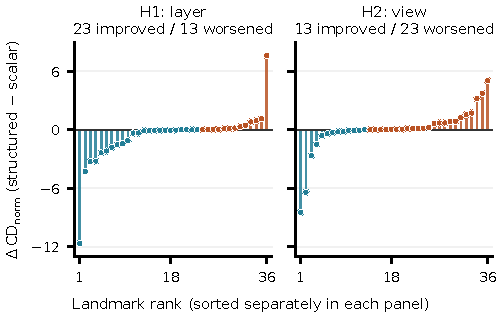
\includegraphics[width=\columnwidth]{figures/point3_h1_h2_confirmation.pdf}
\caption{Paired differences against the scalar for 36 landmarks. Panels are sorted independently; matching ranks need not be the same landmark. Negative favors the structured rule.}
\Description{Two panels use the same vertical scale. H1 has 23 negative differences and 13 positive differences; H2 has 13 negative and 23 positive. H1's mean difference is minus 0.62241; H2's is plus 0.00394.}
\label{fig:structured-confirmation}
\end{figure}

These single-seed, two-candidate studies do not establish statistical significance or full-benchmark generalization. The 79-landmark holdout is untouched; H3 is unfinished. Results, frozen selections, and reproduction scripts are archived with the report.

\section{Challenges and Next Steps}
We will finish H3, review masks and intervention traces, and repeat H1/H2 across seeds. Code and run instructions are in the linked experiment branch (PR \#4).

At the final stage, we will use the whole ArchWorld dataset: all 396 landmarks. Method choices will be frozen on the 317 development landmarks before evaluating the 79 held-out landmarks. We will report held-out scores separately from full-dataset aggregates and provide region/type breakdowns. The per-landmark view protocol still applies; all-landmark coverage does not require every source photo in one reconstruction.

\section{Project Ownership}
\begin{itemize}
\item \textbf{Eric Lu} owns the baseline without intervention, comparison of evaluation pipelines, extraction of Pass-1 features, and feature-based strength selection (Sections~\ref{sec:eric}--\ref{sec:eric-pass1}).
\item \textbf{Swati Parida} owns scene-level adaptive strength selection: the candidate-strength sweep, label-free proxy analysis, depth-drift rule, and development/test evaluation (Section~\ref{sec:swati}).
\item \textbf{Anastasios Gerasis} owns the study of structured interventions: the 54-landmark subset and representativeness audit, shared mask preparation, layer-, view-, and anchor-dependent methods, and the three hypothesis notebooks with matched evaluation and completed H1/H2 analyses (Sections~\ref{sec:point3}--\ref{sec:point3-results}).
\end{itemize}

\bibliographystyle{ACM-Reference-Format}
\bibliography{references}
\end{document}
